\documentclass[UTF8,a4paper,12pt]{ctexbook}

%设置页边距
\usepackage{geometry}
\geometry{left=30mm,right=30mm,top=30mm,bottom=30mm}

%设置英文字体
\usepackage{fontspec}
\setmainfont{Times New Roman}

%设置中文字体
\usepackage{xeCJK}
%\CJKfamily{song}
%\setCJKfamilyfont{st}{宋体}
\newcommand{\st}{\CJKfamily{st}}

%设置字体大小
%\usepackage{type1cm}
%\fontsize{12pt}{}

%设置行间距
\usepackage{setspace}
\setlength{\baselineskip}{20pt}

\usepackage{titlesec}
%\setcounter{secnumdepth}{4}
\titleformat{\chapter}[block]{\LARGE\bfseries\centering}{}{1em}{}
\titleformat{\section}[block]{\Large\bfseries}{\thesection}{1em}{}
\titleformat{\subsection}[block]{\Large\bfseries}{\thesubsection}{1em}{}
%\titleformat{\subsubsection}[block]{\large\bfseries}{\thesubsubsection}{1em}{}
%\titleformat{\paragragh}[block]{\large\bfseries}{\theparagraph}{1em}{}
%\titleformat{\subparagragh}[block]{\large\bfseries}{\thesubparagraph}{1em}{}

%插入图片
\usepackage{graphicx}
\graphicspath{{figures/}}

%设置页眉页脚页码
\usepackage{fancyhdr}
\pagestyle{fancy}
\fancyhead{}% 清除原样式
\fancyhead[CO]{电子科技大学学士学位论文}
\fancyhead[CE]{你好}
\cfoot{\thepage}

%插入伪代码
\usepackage{algorithm, algorithmic}
\usepackage{algpseudocode}  
\usepackage{amsmath}  

\usepackage{listings}


\begin{document}
%单倍行距
%\begin{spacing}{1.0}%%

	
	
\begin{center}
	\Large{\textbf{摘\ 要}}
\end{center}

随着大规模电子商务行业中数据传输量的增加,管理如此大量的请求成为一个关键问题。通过在分布式服务器系统上应用任务调度来处理请求是一种有效的方法。但是,当服务器节点在短时间内处理极大量的请求时,过高负载量是不可避免的。没有有效的高负载监视方法,很难高效的对后端服务器集群进行监控和管理。据我们所知,监控高负载异常节点的现有方法既不灵活也不直观,并且不能检测服务器节点异常,例如定位客户端发送的不合理请求。在本文中,我们提出了一种基于真实数据集的可视化分析的作业调度监控方法,该方法允许监控人员了解该区域中运行节点的状态,并通过各种视图组件观察导致高负载服务器的可疑请求。这种思路为服务器端任务调度集群监测提供了一种全新的方法,并且经过测试显示是可行且有效的。
	
	\textbf{关键词:数据可视化\ 任务调度\ 异常检测}
	%插入空格:\quad或者\ .


%本页不显示页码
\pagenumbering{Roman}
\newpage
%本页不显示页码


\begin{center}
	\large{\textbf{Abstract}}
\end{center}

With the increasing amount of data transmission in large-scale e-commerce industry, managing such an enormous amount of requests simultaneously becomes a key problem. It is an effective method to handle the requests by applying task scheduling on the distributed server system. However, high load on the servers is inevitable in scheduling when requests of a server node process extreme large amount of tasks in a short period of time. It is difficult to maintain load balance without an effective high-load surveillance approach. To best of our knowledge, existing methods of monitoring high-load abnormal nodes are neither flexible or intuitive and are not capable of detecting server node anomalies such as positioning unreasonable requests sent by the clients. In this paper, we propose a job scheduling monitoring method based on visual analysis from a real dataset, which allows the monitoring personnel to know the status of running nodes in the area and observe the suspected requests causing a high load of servers via various view components we inject into the system.

\textbf{Keywords: Task scheduling,\ visual analysis,\ abnormal detection}



\newpage

	
\chapter{第一章\quad 绪\ 论}
\section{研究工作的背景与意义}
现如今网络电子商务项目正在蓬勃发展,人们在享受着足不出户购物和信息浏览,但是往往当使用者的数目变得足够多时,安全隐患往往随之到来。尽管各大互联网企业采取了一些应对措施,比如将用户节点置于类比虚拟机的容器中,或者使用算法对用户请求进行调度处理,使指令被分散在不同的服务器上进行处理,但如果控制这台用户节点的服务器因为某些原因出现超负荷运转,甚至宕机的话,目前整个整个相关领域是没有很好的监视系统来全程监视负责处理用户请求的服务器的运行状态的。比如全球先进的超级计算机研究所——美国德克萨斯州高级计算中心(TACC)现在存在检测正在运行服务器的监视器,但是功能和用户操作流程十分不人性化:他们必须通过具有丰富经验、工作年限很长的后台管理者,通过报错信息得到运行异常的服务器编号,再去监测系统手动输入,通过查看后端返回的一系列运行参数,通过经验判断这台服务器的出错原因从而采取补救措施。类似这样的做法,缺点十分明显,比如在整个操作的过程中,操作流程十分僵硬,充斥着很多人为感知和人为判断,使得操作效率的低下;或者在某一时刻,如果因为在某一地区的用户普遍都出现了系统故障导致在短时间内出现了大面积的服务器运行异常,在如此庞大的工作量之下,工作人员的补救效率在不先进的系统下是很迟钝的,这种中间环节的纰漏就会导致解决过程的滞后,从而引发连带问题。
\section{本文的主要贡献与创新}
本论文的贡献主要是,通过数据可视化手段,实现了对服务器工作状态的全过程实时监测,克服了以前人为操作的种种不利,在功能上也进行了扩充,可以实现的具体功能和创新点如下:
\begin{itemize}
	\item 及时而直观地了解到时间节点下,正常和异常服务器的运行状态参数(CPU利用率、memory利用率、disk利用率等)和服务器本身的各项硬件指标(CPU数目、memory大小等),通过时间和服务器节点实时切换;
	
	\item 通过服务器所带的任务(task)、作业(job)和实例(instance)信息,分析出导致服务器运行异常的原因是由什么任务,或者哪一台用户的异常操作而引起的,在可视化视图中分析异常原因;
	
	\item 直观地观察到服务器任务(task)、作业(job)和实例(instance)之间的包含关系和数目大小,及时得到主要占用服务器资源的作业信息,做出相应调整;
	
	\item 通过热力图刷新迅速掌握某服务器节点在过去一段时间的工作状态,帮助工作人员寻找规律,辅助判断异常节点的出错动机;
	
	\item 了解到在整个有记录的时间线上所有服务器节点的运行状态和某一时刻下的全平台的服务器异常数目,定位异常高峰,联动其他组件有针对性地确定需要观察的时刻。

\end{itemize}
	
总而言之,该方法的创新点就是在传统的监测系统的基础上,通过增加可视化元素,使操作过程变得简洁流畅;在此思路的基础上,增加了各种功能,来帮助监测人员合理地定位异常,通过可视手段分析异常原因,定位故障源,从而有效地实时控制服务器的运行状态,为庞大的商业系统的正常运行保驾护航。

\section{本论文的结构安排}
本文的章节结构安排如下:

第一章:绪论部分,简述研究背景和现阶段研究进展,分析需求从而得出需求;

第二章:详细阐述本文的相关研究、研究意义、研究手段、简述数据可视化方法和研究数据集等研究基础;

第三章:分析系统设计思路,按模块化阐述系统的各部分功能,通过操作视图来具体演示系统的工作流程从而实例化分析,并且加入了测试用例来检验我们想法的正确性和系统的可行性;

第四章:全文的总结和归纳,分析系统仍然存在的缺陷,以及对未来工作的展望;

第五章:参考文献

\newpage

	\chapter{第二章\quad 项目意义及背景介绍}
\section{项目意义}
对电子商务任务调度模式下的异常监测的可视化实现,对此类控制平台提出了一种新的思路和方法,也是数据可视化在交叉领域的全新进展。
\subsection{电商集群的规模化}
2018年7月10日,2018中国互联网大会发布了新一版的《中国互联网发展报告(2018)》。报告中指出,2017年,中国电子商务交易服务营收规模为5027亿元,首次突破5000亿大关。2017年第三方互联网支付也达到143.26万亿,网络购物市场交易规模达5.33万亿元,而网络零售的市场交易规模为7.18万亿。中国网上支付用户规模达5.31亿人,其中手机支付用户就达5.27亿人,较2016年底增加5783万人,年增长率为12.3\%,规模增长迅速。正如网民在现实生活中体会到的,电子商务交易已经成为我们购买日常用品的首选手段,在中国庞大的网民基数和中国网络技术飞速发展的双重影响下,这一数字在以后还会以大增幅增长。根据商务部统计,2020年预计中国网络零售市场规模为9.6万亿,是2012年的10倍之多。电子商务在深度影响着国民生活的同时,也掌握着货架经济的命脉,倘若电商集群由于某种原因崩溃的话,给整个国家带来的影响即将是灾难性的。

中国电子商务的龙头企业——阿里巴巴网络技术有限公司(以下简称阿里巴巴),在国内的电子交易平台里扮演着举足轻重的地位。根据2018年阿里巴巴公布的财年财报显示:2018全年,阿里巴巴营收 2502.66 亿元人民币(约 398.98 亿美元),同比增长 58\%,核心电商业务收入 2140.20 亿元人民币,同比增长 60\%,均创下IPO(Initial Public Offerings,指股份公司首次向社会公众公开招股的发行方式,简称IPO)以来年度最高增幅,2018 财年净利润为 832.14 亿元人民币(约 132.66 亿美元)。如此庞大的交易额和成交额使专家和研究人员不自主地将目光放在其身上。2018年阿里巴巴在Github上公布了一组数据,该数据刻画了阿里巴巴在8天地范围内4000台服务器的运行状态的数据,而这组数据也将成为本项目的研究数据集,在本章第三部分,将会着重对该数据进行详细介绍。

\subsection{故障问题及手段}
电子商务平台的实现其实并不是一个不能达到的要求,但是任何系统架构在达到一定规模之后,大大小小的问题往往会接踵而至,而这也是一个企业生存的关键。2018年8月1日,阿里巴巴旗下的淘宝网交易平台,淘宝服务器出现大范围的故障,全国多地网友在微博反馈称自己的淘宝崩溃无法查看订单,淘宝App、PC版网页均出现“网络竟然崩溃了”的提示,即使切换网络和重启手机也无效,在长达数小时的等待之后,该漏洞得到了修复。具体的原因,阿里巴巴并没有给出明确的回复,之后这件事也就不了了之。然而这已经不是阿里巴巴遇到的第一次服务器崩溃事件,每隔数月就会时不时的发生类似的服务器故障。由此可见,即使是如此宏大的电子商务企业也会因为后端服务器的宕机事件,造成企业形象的不良影响的同时也造成了利润的亏损。换句话说,如果能快速发现故障,找出导致该进程异常的原因,再利用分支等手段同时进行维护,结果将会截然不同。而本系统的设计初衷就是以阻止此类问题的发生而提出的。
\subsection{设计优势}
本系统设计将基于可视分析,在对服务器异常进行图形化展示的同时,还拥有异常定位、时序性监测等特点,对出现异常信号的服务器节点进行实时监测,并直观的展示造成该异常的任务,从而达到快速、准确的定位故障的目的。
\section{项目背景及相关理论}
\subsection{研究现状}
{面对异常检测问题}\cite{article2},Xiaowei Qin等人提出了一种{面向对象的检测框架}\cite{article3},它具有两步聚类,称为沙漏聚类。两个参数,关键质量指标和因果参数,通过结合自组织映射(SOM)和k-medoids的混合算法,将它们聚类成不同的类型。{Pei Yang等人}\cite{article4}。建议使用生成的拮抗网络(GAN)来检测异常。{Daojing He等人}\cite{article6},介绍使用软件定义网络(SDN)检测流量异常的优势。A.R.Jakhale\cite{article10}使用{数据挖掘}\cite{article7}\cite{article8}\cite{article9}技术,利用滑动窗口模型和聚类技术检查网络流的异常数据包。 {Alireza Tajary}\cite{article11}等,提出了一种吞吐量感知的瞬态故障检测方法,它利用了多核服务器处理器的特性。

为了识别大型,动态和异构数据中的异常\cite{article14},Nan Cao等,介绍一种视觉互动\cite{article20}\cite{article21}\cite{article22}系统和框架,称为Voila。该系统主要实现在线监测和与用户的互动。{Y.B. Luo等人}\cite{article23},提出了一种基于流量限制可穿透能见度图(FL-LPVG)的异常检测方法。该方法基于网络流序构建复杂网络,挖掘相关图的结构行为模式,提取网络流特征序列,利用LPG将统计特征序列转换为关联图,通过数据挖掘和信息检测异常流量基于熵的理论技术。其优点是该方法大大简化了异常检测过程,有效降低了高维数据的维数。但是为了提高这个系统的效率,我们必须从大量数据中完全挖掘行为特征。因此,它肯定会带来如何处理大数据以及如何提取有效信息的挑战。

{Josef Kittler 等人}\cite{article27},在解决异常检测问题时引入{域异常的概念}\cite{article24}\cite{article25}。异常有许多方面,每个域都是异常的许多方面之一。在此基础上,他们参考贝叶斯概率推理设备,并提出统一的{异常检测框架}\cite{article26},以识别和区分每个领域的异常。该设备通过定义各种异常属性来提供域异常事件的分类。该框架的创新特点是它暴露了异常的多方面性质,并且可以识别可能导致异常事件的各种原因,以及相应的检测机制。

\subsection{数据可视化}
本项目的特征是基于数据可视化的电商平台集群管理。数据可视化是由于视觉给人类带来的感知是最直观最有效率的一种获取信息的手段。目前国内的数据可视化行业也在蓬勃发展,涌现除了不少有能力的人才和惊艳的科技成果,下面将用一小部分篇幅来介绍一下这门领域的相关特点及其主要用途。

从生物学的角度来考虑,人类所有器官能接收到信息的80\%都来自于视觉,在大数据时代下,对信息的表达则就显得尤为关键,而数据可视化也就承担起了这一重要任务,充当着数据和人类之间的关键载体。顾名思义,数据可视化是关于数据视觉表现形式的科学技术研究。其中,这种数据的视觉表现形式被定义为,一种以某种概要形式抽提出来的信息,包括相应信息单位的各种属性和变量。它是一个处于不断演变之中的概念,其边界在不断地扩大。主要指的是技术上较为高级的技术方法,而这些技术方法允许利用图形、图像处理、计算机视觉以及用户界面,通过表达、建模以及对立体、表面、属性以及动画的显示,对数据加以可视化解释。
\subsection{电子商务分布式任务调度}
作业调度是用于控制作业的无人值守后台程序执行的计算机功能,也称为批量调度。作业调度程序需要协调实时业务活动与跨不同操作系统平台和业务应用程序环境的传统后台IT处理的集成。作业调度程序需要通过几个参数管理客户端计算机集群的作业队列,例如作业优先级,计算机源可用性或用户允许的同时作业数。这种作业调度方法已成为大型电子商务业务平台处理用户并发请求的常用方法。

\begin{figure}
	\centering
	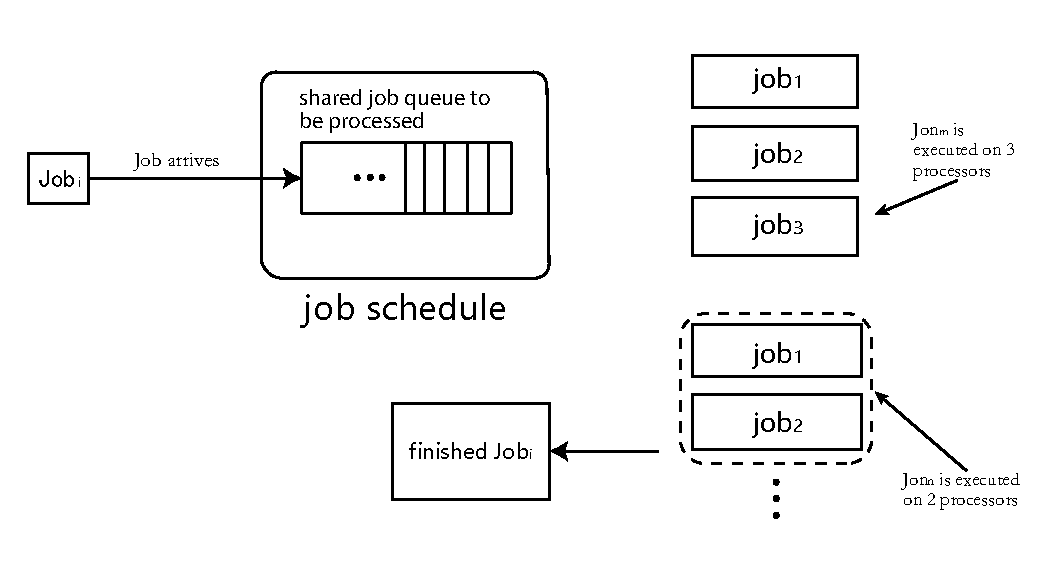
\includegraphics[height=0.45\textwidth]{52}
	\caption{作业调度模型}
	\label{fig-1}
\end{figure}

图\ref{fig-1}说明了本文假设的作业调度程序模型。在该图中,用户提交的作业到达共享作业队列,并且作业调度器获得作业请求的处理器的数量(job大小)。没有给作业调度程序提供其他信息。作业调度程序收集处理器的状态,空闲或忙碌,并将共享作业队列中的作业分派给空闲处理器。这里有两个执行作业的策略。在第一个策略中,作业调度程序将作业调度到S处理器,并保证在S处理器上执行作业直到完成。这里,S表示工作规模。在第二个策略中,作业调度程序不保证在S处理器上执行作业,也就是说,执行作业的处理器数量取决于并行计算机上作业的拥塞程度。在第一个策略中执行的作业称为刚性作业。

同时,一旦操作员处理了工作流程被实例化,它就被称为“任务”。实例化在调用抽象运算符时定义特定值,参数化任务成为DAG中的节点。基于该层处理,任务被分成几个部分,可以分派到服务器进行处理,这通常称为“任务实例”。任务实例表示任务的特定运行,其特征在于标记,任务和时间点的组合。由于流程的抽象和复杂性,图\ref{fig-2}向我们展示了如何作业实例将逐步拆分为任务实例。

\begin{figure}[htbp]
	\centering
	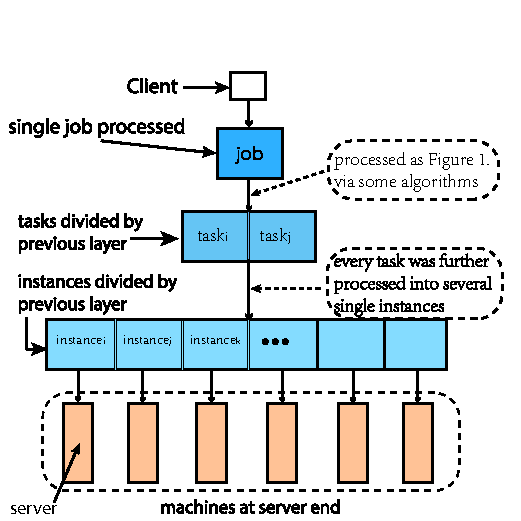
\includegraphics[height=0.55\textwidth]{5}
	\caption{来自作业层的工作流程型}
	\label{fig-2}
\end{figure}
\subsection{数据集分析}
本研究中使用的数据集cluster-trace-v2018\footnote{\ https://github.com/guanxyz/clusterdata/blob/master/cluster-trace-v2018/trace\_2018.md}将从我们的一个生产集群中进行跟踪和采样,cluster-trace-v2018是Alibaba Open Cluster Tracking Program\footnote{\ 阿里巴巴集群跟踪计划由阿里巴巴集团出版。通过提供来自实际生产的集群跟踪,该计划帮助研究人员,学生和对该领域感兴趣的人更好地了解现代互联网数据中心(IDC)和工作负载的特征。https://github.com/guanxyz/clusterdata}的一部分。该计划由阿里巴巴集团发布,并于2017年提出并开始跟踪。通过实际生产提供集群跟踪,该计划帮助研究人员,学生和对该领域感兴趣的人更好地了解现代互联网数据中心的功能和工作量(ID)。该项目目前已在Version 2017\footnote{\ https://github.com/guanxyz/clusterdata/tree/master/cluster-trace-v2017}和2018版本中提供。 2017版本是该程序的原型,它记录了3000个服务器节点的12小时跟踪。为了研究的全面性和完整性,我们打算在2018年版的基础上进行研究。cluster-trace-v2018包括大约4000台机器,跨时8天,由6个单独的数据文件组成,数据文件总大小达到了206GB,以下是该数据集的简要介绍:
\begin{itemize}
	\item machine\_meta:机器的元信息和事件信息。
	\item machine\_usage:每台机器的资源使用情况。
	\item containe\_meta:容器的元信息和事件信息。
	\item container\_usage:每个容器的资源使用情况。
	\item batch\_instance:有关批处理工作负载中实例的信息。
	\item batch\_task:有关批处理工作负载中实例的信息。
\end{itemize}

以上六个数据集在空间性上和时序性上向我们充分展示了每台服务器的信息、运行情况以及服务器所接受的任务调度,横向和纵向的展示了在为其8天的事件范围内所有任务的调度情况以及接受这些调度的机器的运行状态。
\section{关键问题}
\subsection{数据处理}
由于研究所采用的数据集十分庞大,故成为了本项目进行的一大难题。用以往的方法去分析和处理该数据集并不是最理想的手段,比如将整个数据读入内存然后进行处理,或者将数据按时序拆分成多个数据文件在单独进行处理。前者不可行的原因是实验地点的硬件条件还不能满足将如此庞大的数据这个整个读入内存,这必将造成计算机内存过载导致系统崩溃,而后者也不是最理想化的解决办法,因为比如将数据文件按天数切割成8份,每一份的文件大小也将达到15GB,即使可以读入内存但是也造成了内存占用率过高从而导致其他进程无法正常运行。

在另一方面来说,假设我们用某种方法将数据成功的导入了我们指定的数据库,但是在后台与数据库交互的过程中,由于查询的数据量过于庞大,会导致超出后台数据接口所能容纳的数据量最大限额,导致查询时间过慢或者因为超出接口限额请求时间过长而进程中断导致程序崩溃。

综上所述,以上两个难点都是因为数据量的规模所导致的问题,所以如何处理大数据量的数据集是本次项目亟待解决的一个难点。
\subsection{集群表示及定位故障源}
如何将任务(job)、作业(task)和作业实例(instance)(以下分别简称job、task和instance)与运行节点通过可视化手段巧妙地结合起来将成为一个有价值的话题。按照传统方法,先将所有节点与其运行状态在一个视图中表示出来,再通过交互使之与另一数据表中的job等参数链接起来,虽然可行但是再操作的过程中略显繁琐。而且根据数据文件的特征,决定了不能从节点使用情况的视图出发去查询作业实例等信息,两者的数据文件中的时间戳存在被包含的关系,所以不能用传统机械的方法去处理本项目的数据结构。

该关系可以大致归纳为一个树形结构,job、task与instance从前往后依次存在包含关系,而对于每一个instance都有一台独立的服务器节点用来处理该instance所发出的请求。该请求的分布可能是分布式的,这就导致了通一个job下所包含的instances被调度到了不同的节点来进行处理,所谓分布式任务调度。

值得注意的是,用户节点与job之间只存在一对多的关系,不存在不同用户所调度的job属于同一个job,这一点十分关键,在第三章第一节将具体分析此数据结构的特点。
\subsection{故障域算法}
用来判断硬件性能的算法不少,但是用于检测服务器负载异常的算法却不多见,而且使用范围有限。大规模服务器集群的异常确定算法类似于云计算基础设施中异常识别的处理模式。 该方法,最相关的主成分(MRPC)\footnote{\ Most relevant procedure component},由于缺乏动态规范化单位和规模的关键参数,因此无法应用于我们的研究。 
\subsection{时序性及空间性}
在研究目标为实时性的要求下,对时序性的反映往往是至关重要的。采用数据库的目的是可以实时对数据库内的记录进行可视化输出,然而这还远远不够,我们需要通过节点的过往记录和对未来节点运行状态的预测来具有时效性的描述节点,这样管理者不但可以从视图的渲染中找到异常规律从而在以后有针对性的操作节点,还可以对未来节点的运行状态进行预测,适当关闭或者限流问题节点从而对整个服务器集群和用户端的操作进行优化和改进。

在布局的空间性问题上,往往要在有限个数的可控维度上尽可能多的表示信息,所以节点的空间性排布成为一个值得商榷的问题。按照团队的初步设想,将节点表示为具有时序性的三维排布,每个维度各自表示判定异常的相关参数(CPU利用率、memory利用率、disk利用率),但这样做的成果其实并不理想:使用者并不关心每个节点的异常参数,所以对维度的利用是一种浪费,不符合可视分析的规范。
	\chapter{第三章\quad 系统设计与实现}
\section{项目意义}
\subsection{主要任务}

为了解决现有任务调度控制方法的不人性化和不直观以及拓展更多功能的需求,故提出本项目,旨在为解决以上问题而更近一步。具体任务列举如下:

\begin{itemize}
	\item 通过可视化分析的方法及时地了解到某时间节点下,正常和异常服务器的运行状态参数(CPU利用率、memory利用率、disk利用率等)和服务器本身的各项硬件指标(CPU数目、memory大小等),并且可以进行实时切换的功能;
	\item 通过调度信息(task、job和instance),由图形展示出导致异常的原因归咎于哪个具体task或job,由此得到用户操作对后端服务器的影响;
	\item 直观看到服务器任务(task)、作业(job)和实例(instance)之间的包含关系以及数目大小,得到主要占用服务器资源的作业信息,做出相应调整;
	\item 通过热力图刷新迅速掌握某服务器节点在过去一段时间的工作状态,帮助工作人员寻找规律,辅助其他模块判断异常节点的出错动机;
	\item 了解到在某一时间点下拥有记录的所有服务器节点的运行状态和该时间下运行某任务的服务器异常数目,定位异常高峰,并由此有针对性地确定需要观察的时刻。
\end{itemize}

本文拟根据以上需求设计并实现相应的系统模块,设计和实现过程在本章的余下章节将展开详细说明。

%\newpage
\subsection{关键问题的解决方法}

{\textbf{3.1.2.1\quad 数据处理}}

上文中提到,处理、读取并查找庞大量级的数据文件成为了一大难题。出于对本项目模型性和实时性的考虑,经过团队的讨论最终决定选择八天中第二天的数据作为数据集模拟数据流进行研究。然而问题是经过分割后的数据文件的体积仍然超过了研究地点所有独立设备的内存极限,解决方法在于python对数据处理方法的改变:如算法\ref{alg-1}所示,改变以往的处理中小型数据的思路和方法,将庞大的数据集每次按需读入设备内存进行处理,故得出两种可行的方法,python csv中的按行读取方法和pandas的块级读取的方法,即每次根据电脑内存大小只读取原数据文件的一小部分,等这一部分被处理和计算结束后再去重复操作处理其他部分的数据。这样便实现了任意大小的文件都可以被任意设备进行处理和计算的方法。

\begin{algorithm}
	\caption{Huge data file reade}
	\label{alg-1} 
	\textbf{Input}: data\_path
	
	1:\textbf{initialize}:reader=csvReader(data\_path)
	
	2:\textbf{for} row  \textbf{in} reader do
	
	3:\qquad filter by Conditions
	
	4:\qquad write(row)
	
	5:\textbf{end for}

\end{algorithm}

{\textbf{3.1.2.2\quad 集群表示及定位故障源}}

为了准确而简洁地表示每一个任务所持有的job、task与instance参数,以及如何将三者与具体被调度地服务器节点联系起来,经过讨论拟采用以下方案:采用可是分析展示方法中的tree结构,可以清晰明了地展示三者之间地层次关系。与此同时,在叶子节点的节点处与相应处理服务器绑定,反映正在运行此instance的服务器所处的运行状态。通过以上方法,就完美解决了任务调度信息的层次关系和不同数据文件之间的关联。

{\textbf{3.1.2.3\quad 故障域算法}}

数据集本身有许多参数来说明后端服务器节点的状态。 控制阈值是确定异常域的有效方法,取决于三个有价值的领域:CPU利用率,内存利用率和磁盘利用率。 通过为这三个参数分配权重,系统可以确定节点在处理任务实例时是否处于高负荷。 算法二描述了在我们的研究中识别异常的方法:

$$Value_{hl}=x\cdot\frac{S_{\beta +\gamma}}{S}+y\cdot\frac{S_{\alpha+\gamma}}{S}+z\cdot\frac{S_{\alpha+\beta}}{S}$$

在上面的算法中,$\alpha$,$\beta$和$\gamma$分别代表CPU,内存,磁盘的阈值。 我们使用概率统计学的思想来设置适当的阈值,以保持异常高负荷节点的比例接近10%。 可以像这样计算高负荷的负荷值。

{\textbf{3.1.2.4\quad 时序性及空间性}}
为了将数据可视化与节点状态的时序性结合起来,我们拟通过日历图的热力排布来展示一个服务器节点在过去一段时间内的运行状态。通过像素块颜色的深浅,直观反映某节点的健康程度。

由于缺少节点的地理位置信息,所以不能将集群的地理分布在地图上展示,前期拟定的三维数值坐标展示将只用树状结构叶子节点的热力色块来展示。因为使用者并不用清楚的知道此时此刻服务器的各种利用率参数,只需要知道该节点健康与否即可。
	
	\begin{thebibliography}{99}

		\bibitem{article2}J. Al Dallal, P. Sorenson, “System testing for object-oriented frameworks using hook technology”, Proceedings 17th IEEE International Conference on Automated Software Engineering, 2002.
		
		\bibitem{article3}Xiaowei Qin, Shuang Tang, Xiaohui Chen, Dandan Miao, Guo Wei, “SQoE KQIs anomaly detection in cellular networks: Fast online detection framework with Hourglass clustering”, China Communications, pp.25-37, 2018.
		
		\bibitem{article4}Pei Yang, Weidong Jin, Peng Tang, “Anomaly Detection of Railway Catenary Based on Deep Convolutional Generative Adversarial Networks”, 2018 IEEE 3rd Advanced Information Technology, Electronic and Automation Control Conference (IAEAC), 2018.
				
		\bibitem{article6}Daojing He, Sammy Chan, Xiejun Ni, Mohsen Guizani, “Software-Defined-Networking-Enabled Traffic Anomaly Detection and Mitigation”, IEEE Internet of Things Journal, 2017.
		
		\bibitem{article7}Vania Bogorny, Shashi Shekhar, “Spatial and Spatio-temporal Data Mining”, 2010 IEEE International Conference on Data Mining, 2010.
		
		\bibitem{article8}Hetal Thakkar, Barzan Mozafari, Carlo Zaniolo, “A Data Stream Mining System”, 2008 IEEE International Conference on Data Mining Workshops, 2008.

		\bibitem{article9}G. Williams, R. Baxter, Hongxing He, S. Hawkins, Lifang Gu, “A comparative study of RNN for outlier detection in data mining”, 2002 IEEE International Conference on Data Mining, 2002. Proceedings, 2002.
		
		\bibitem{article10}A. R. Jakhale, “Design of anomaly packet detection framework by data mining algorithm for network flow”, 2017 International Conference on Computational Intelligence in Data Science (ICCIDS), 2017.
		
		\bibitem{article11}Alireza Tajary, Hamid R. Zarandi, “An Efficient Soft Error Detection in Multicore Processors Running Server Applications”, 2016 24th Euromicro International Conference on Parallel, Distributed, and Network-Based Processing (PDP), 2016.
		
		\bibitem{article14}Chihiro Sakazume, Hiroyuki Kitagawa, Toshiyuki Amagasa, “DIO: Efficient interactive outlier analysis over dynamic datasets”, 2017 Twelfth International Conference on Digital Information Management (ICDIM), 2017.

		\bibitem{article20}Nan Cao, Chaoguang Lin, Qiuhan Zhu, Yu-Ru Lin, Xian Teng, Xidao Wen, “Voila: Visual Anomaly Detection and Monitoring with Streaming Spatiotemporal Data”, IEEE Transactions on Visualization and Computer Graphics, pp. 23 – 33, 2018.
		
		\bibitem{article21}Cheong Hee Park, “Anomaly Pattern Detection on Data Streams”, 2018 IEEE International Conference on Big Data and Smart Computing (BigComp), 2018.
		
		\bibitem{article22}Li Xinran, “Research on massive data 3D-visualization”, 2012 IEEE International Conference on Computer Science and Automation Engineering, 2012.
		
		\bibitem{article23}Y.B. Luo, B.S. Wang, Y.P. Sun, B.F. Zhang, X.M. Chen, “FL-LPVG: An approach for anomaly detection based on flow-level limited penetrable visibility graph”, 2013 International Conference on Information and Network Security (ICINS 2013), 2013.
		
		\bibitem{article24}Hongbin Xia, Wenbo Xu, “Research on Method of Network Abnormal Detection Based on Hurst Parameter Estimation”, 2008 International Conference on Computer Science and Software Engineering, 2008.
		
		\bibitem{article25}Zhixin Sun, Jin Gong, “Anomaly Traffic Detection Model Based on Dynamic Aggregation”, 2010 Third International Symposium on Electronic Commerce and Security, 2010.
		
		\bibitem{article26}Yong Li, Wei-Yi Liu, “Backward probabilistic logic reasoning algorithm for decision problem with Conditional Event ALgebra on Bayesian networks”, 2008 International Conference on Machine Learning and Cybernetics, 2008.
		
		\bibitem{article27}Josef Kittler, William Christmas, Teófilo de Campos, David Windridge, Fei Yan, John Illingworth, Magda Osman, “Domain Anomaly Detection in Machine Perception: A System Architecture and Taxonomy”, IEEE Transactions on Pattern Analysis and Machine Intelligence, pp.845-859, 2014.

		
	\end{thebibliography}
	
\end{document}